\documentclass[a4paper]{article}
% Preamble
\usepackage[utf8]{inputenc}
\usepackage{fullpage}
\usepackage[english]{babel}
\usepackage{color}
\usepackage{amsmath}
\usepackage{url}
\usepackage{standalone}
\usepackage{parskip}
\usepackage{graphicx}
\usepackage{caption}
\usepackage{subcaption}
\usepackage{natbib}
\usepackage{amsfonts}

\title{Tensor Calculus - Faculty of Khan}
\author{Lauren Shriver}
\date{Summer 2019}

\begin{document}
\maketitle

\section{Introduction to Tensors}
\textbf{Scalars} = quantities that only have magnitude
    \begin{itemize}
        \item Specify with 1 component and 0 basis vectors
        \item Example: Temperature
    \end{itemize}
\textbf{Vectors} = quantities that have a magnitude and one direction
    \begin{itemize}
        \item Specify with $n$-components and $n$-basis vectors (one basis vector per component) 
        \item Example: Displacement vector $\mathbf{a} = a_1\mathbf{\hat{e}_1} + a_2\mathbf{\hat{e}_2} + a_3\mathbf{\hat{e}_3}$ in 3D space
            \begin{itemize}
                \item Three components: $a_1$, $a_2$, and $a_3$
                \item Three basis vectors: $\mathbf{\hat{e}_1}$, $\mathbf{\hat{e}_2}$, and $\mathbf{\hat{e}_3}$
                \item Magnitude: $a=\mathbf{|a|}=\sqrt{(a_1)^2 + (a_2)^2 + (a_3)^2}$
                \item Example: Stress tensor
            \end{itemize}
    \end{itemize}
\textbf{Dyads} = quantities that have a magnitude and two directions 

    
 
    \begin{itemize}
        \item Specify with $n^2$-components and $n^2$-basis vectors
        \item Example: Stress applied at a point in 3D space (see \ref{fig:stress})
        \begin{itemize}
            \item Consists of 9 componenents, each of which is specified using two basis vectors 
            \begin{equation}
                P = \left[
                    \begin{array}{ccc}
                         P_{xx} & P_{xy} & P_{xz} \\
                         P_{yx} & P_{yy} & P_{yz} \\
                         P_{zx} & P_{yz} & P_{zz}
                    \end{array}
                    \right]
            \end{equation}
                \begin{figure}[h!]
    \centering
            
    \begin{subfigure}[b]{0.3\linewidth}
        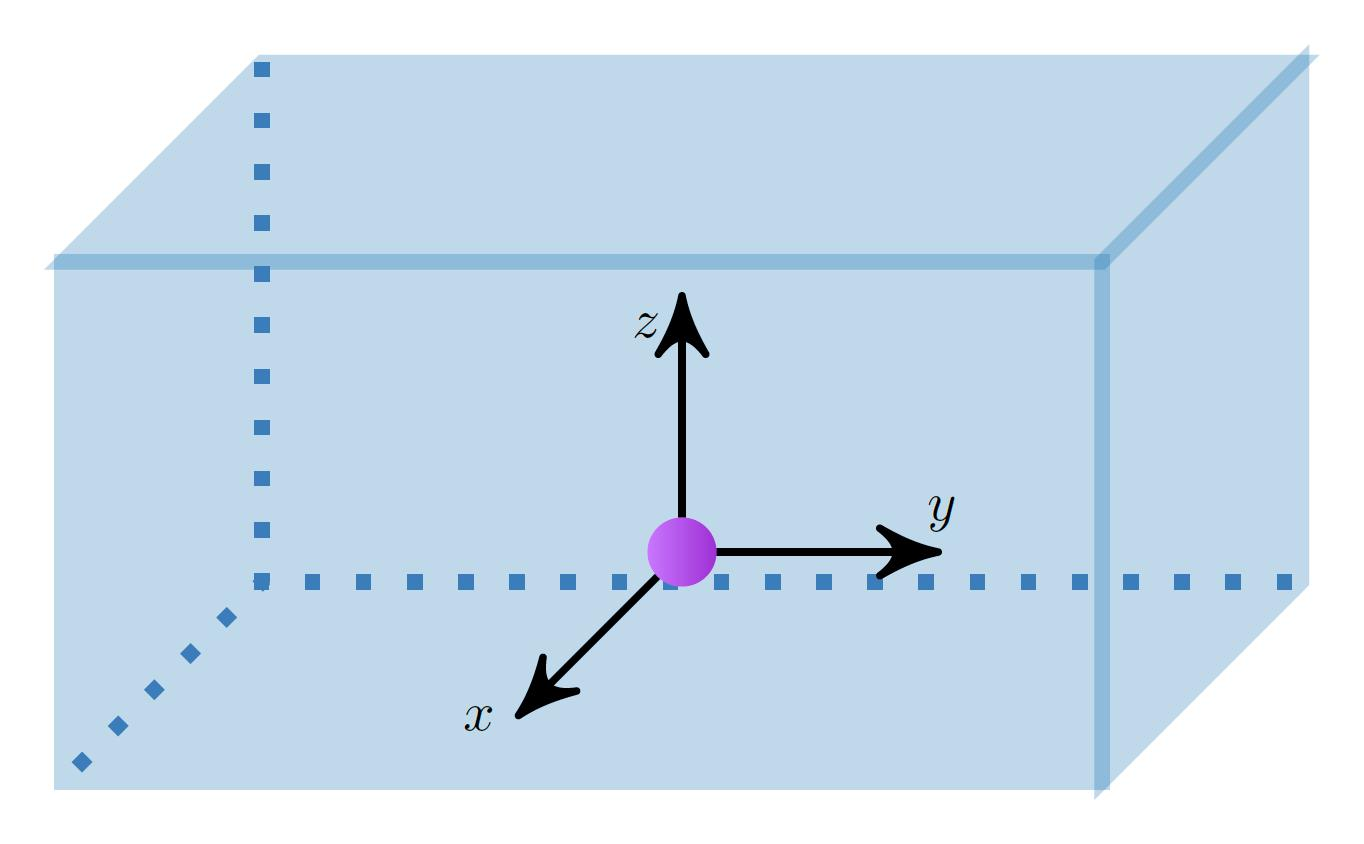
\includegraphics[width=\linewidth]{Images/Stress_Tensor_Images/stress1.jpg}
            \caption{Point in a beam}
        \end{subfigure}
        \\
        \begin{subfigure}[b]{0.3\linewidth}
            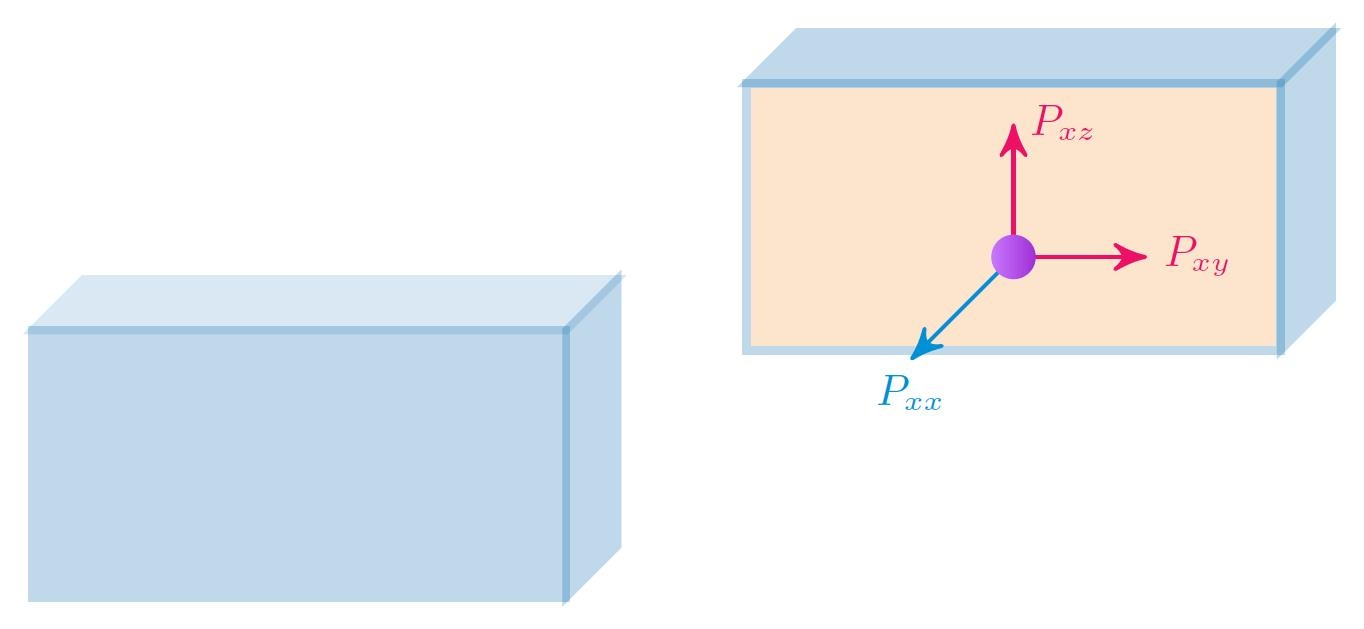
\includegraphics[width=\linewidth]{Images/Stress_Tensor_Images/stress2.jpg}
            \caption{Components defined with respect to the $x$-face}
        \end{subfigure}
        \begin{subfigure}[b]{0.3\linewidth}
            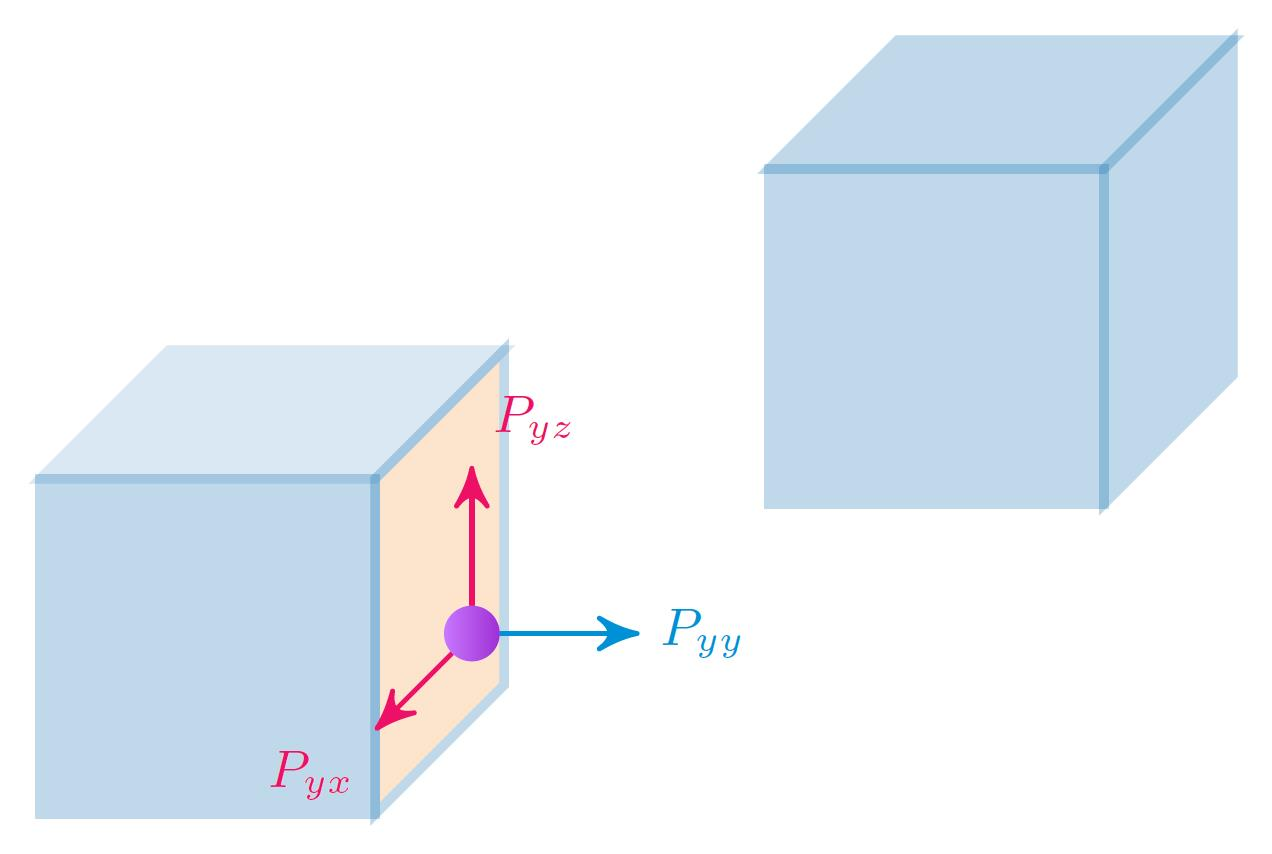
\includegraphics[width=\linewidth]{Images/Stress_Tensor_Images/stress3.jpg}
             \caption{Components defined with respect to the $y$-face}
        \end{subfigure}
        \begin{subfigure}[b]{0.3\linewidth}
            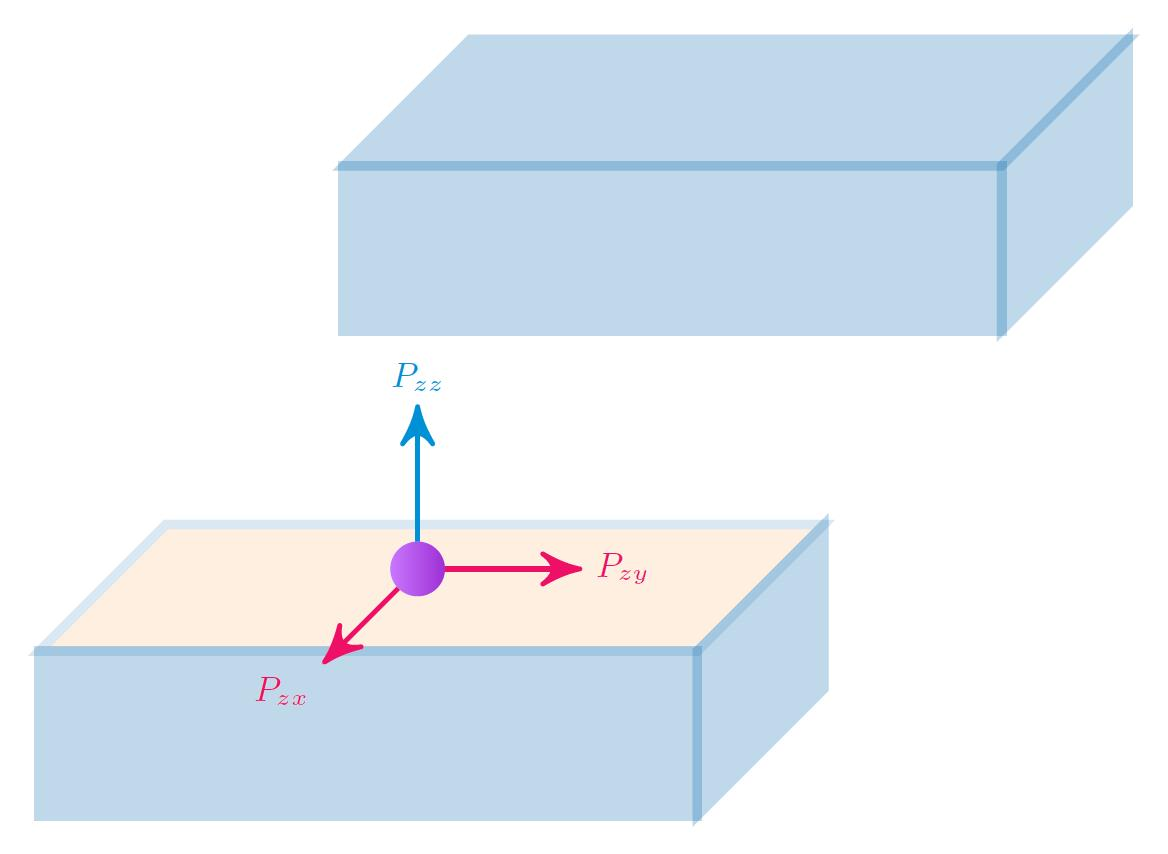
\includegraphics[width=\linewidth]{Images/Stress_Tensor_Images/stress4.jpg}
            \caption{Components defined with respect to the $z$-face}
        \end{subfigure}
        
        \caption{Stess Tensor}
        \label{fig:stress}
    \end{figure}
            \item For each component $P_{ij}$, 
            \begin{itemize}
                \item The $i$ index denotes the cross-sectional face perpendicular to a given pulling force (or parallel to a given shearing force)
                \begin{itemize}
                    \item Q: Does $i$ technically represent a bivector?
                \end{itemize}
                \item The $j$ index denotes the direction of a given force
            \end{itemize}
            \item Each component has units in force per area (e.g., $\mathrm{N}/\mathrm{m}^2$)
            \item 
        \end{itemize}
    \end{itemize}      
\end{document}

